\chapter{Scenariile de testare}

Suita de teste acoperă șase fluxuri end-to-end, alese astfel încât să reprezinte parcursurile
critice ale unui utilizator real pe o platformă de e-commerce. Fiecare scenariu este descris
prin precondiții, pași de testare și aserțiuni, însoțit de diagrama fluxului de execuție.

Notație utilizată în diagrame:
\begin{itemize}
    \item \textbf{Acțiune} --- interacțiune directă cu interfața (click, completare formular, navigare);
    \item \textbf{Aserțiune} --- verificare că sistemul se află în starea așteptată;
    \item \textbf{Soft assert} --- verificare opțională; eșecul este înregistrat, dar testul continuă.
\end{itemize}

% -------------------------------------------------------
\section{Workflow 1 --- Cumpărături ca vizitator (Guest mega-flow)}

\subsection*{Precondiții}
\begin{itemize}
    \item Sesiune de browser nouă (incognito), fără cont activ.
    \item Coșul de cumpărături și wishlist-ul sunt goale.
\end{itemize}

\subsection*{Pași de testare}
\begin{enumerate}
    \item Navigare prin meniu și aplicarea unui filtru asincron (16 GB RAM) pe categoria Notebooks.
    \item \textbf{Assert}: răspunsul AJAX de filtrare returnează HTTP 200.
    \item Adăugarea primului produs afișat în wishlist.
    \item \textbf{Assert}: notificarea verde de confirmare este vizibilă.
    \item Transferul produsului din wishlist în coș, actualizarea cantității la 2.
    \item \textbf{Assert}: prețul total este exact dublul prețului unitar.
    \item Checkout ca vizitator: completare adresă de facturare, selectare livrare \textit{Next Day Air}, plată cu card.
    \item \textbf{Assert}: URL-ul final conține \texttt{/checkout/completed}.
    \item \textbf{Assert}: titlul paginii este \textit{``Your order has been successfully processed!''}.
\end{enumerate}

\begin{figure}[H]
    \centering
    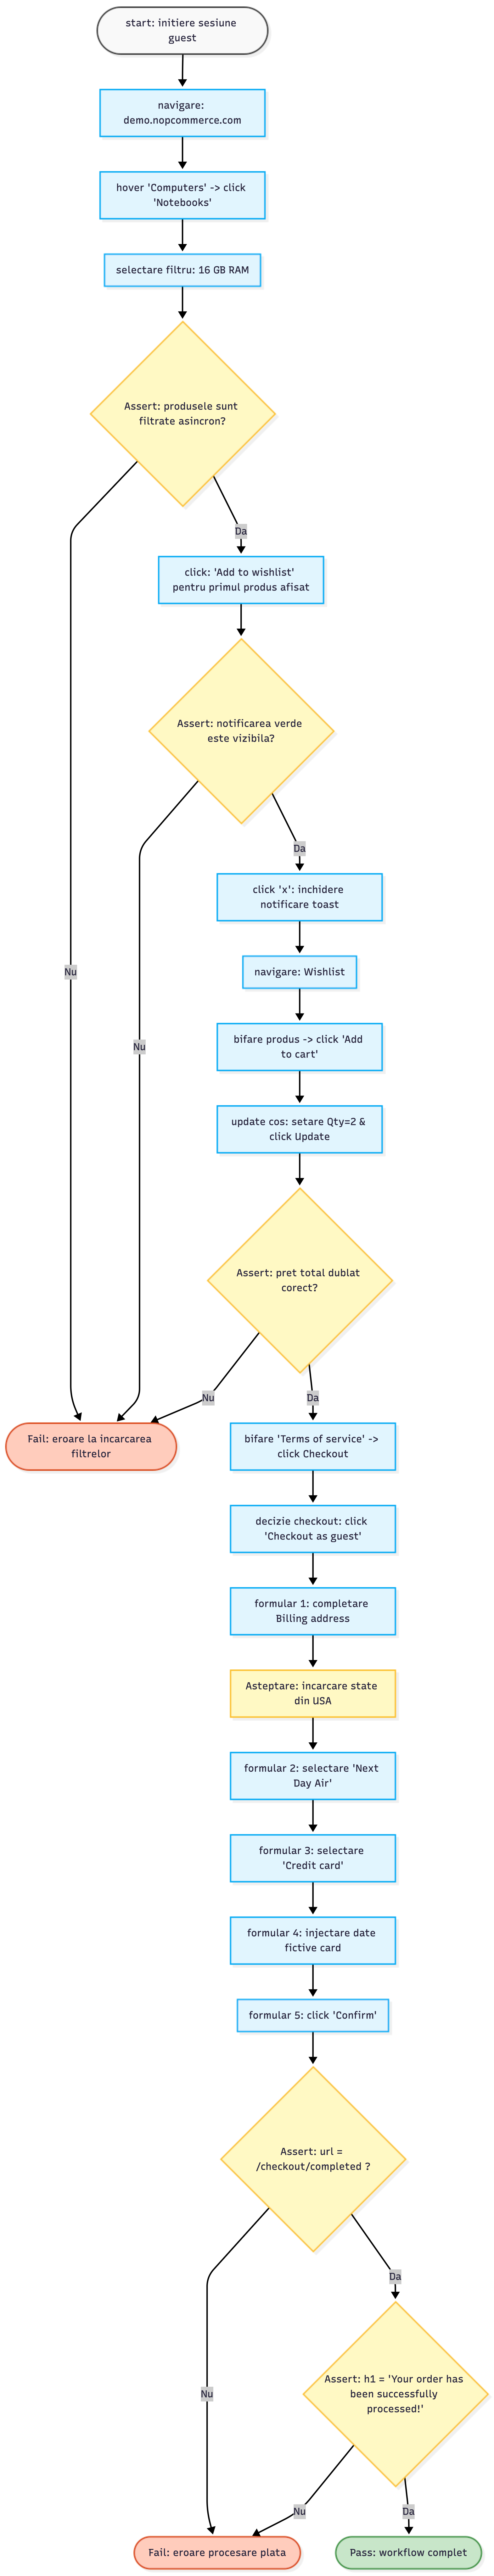
\includegraphics[width=0.3\textwidth]{diagrams/diagram1.png}
    \caption{Diagrama fluxului --- Workflow 1: Guest mega-flow}
    \label{fig:wf1}
\end{figure}

% -------------------------------------------------------
\section{Workflow 2 --- Configurator PC cu prețuri dinamice}

\subsection*{Precondiții}
\begin{itemize}
    \item Sesiune guest, coș gol.
\end{itemize}

\subsection*{Pași de testare}
\begin{enumerate}
    \item Schimbarea valutei la Euro.
    \item \textbf{Assert}: simbolul \euro{} apare pe prețurile afișate.
    \item Navigare la produsul \textit{Build your own computer}; extragerea prețului de bază.
    \item Selectare dinamică de componente (RAM, HDD, software) cu interceptare răspunsuri AJAX.
    \item \textbf{Assert}: noul preț este mai mare decât prețul de bază.
    \item Adăugare în coș; aplicarea cuponului invalid \texttt{cupon-fals-2026}.
    \item \textbf{Soft assert}: mesajul de eroare roșu este vizibil; testul continuă indiferent.
    \item Checkout cu adresă de livrare diferită de cea de facturare.
    \item Selectare metodă de plată \textit{Check/Money Order}.
    \item \textbf{Assert}: mesaj de confirmare a comenzii.
\end{enumerate}

\begin{figure}[H]
    \centering
    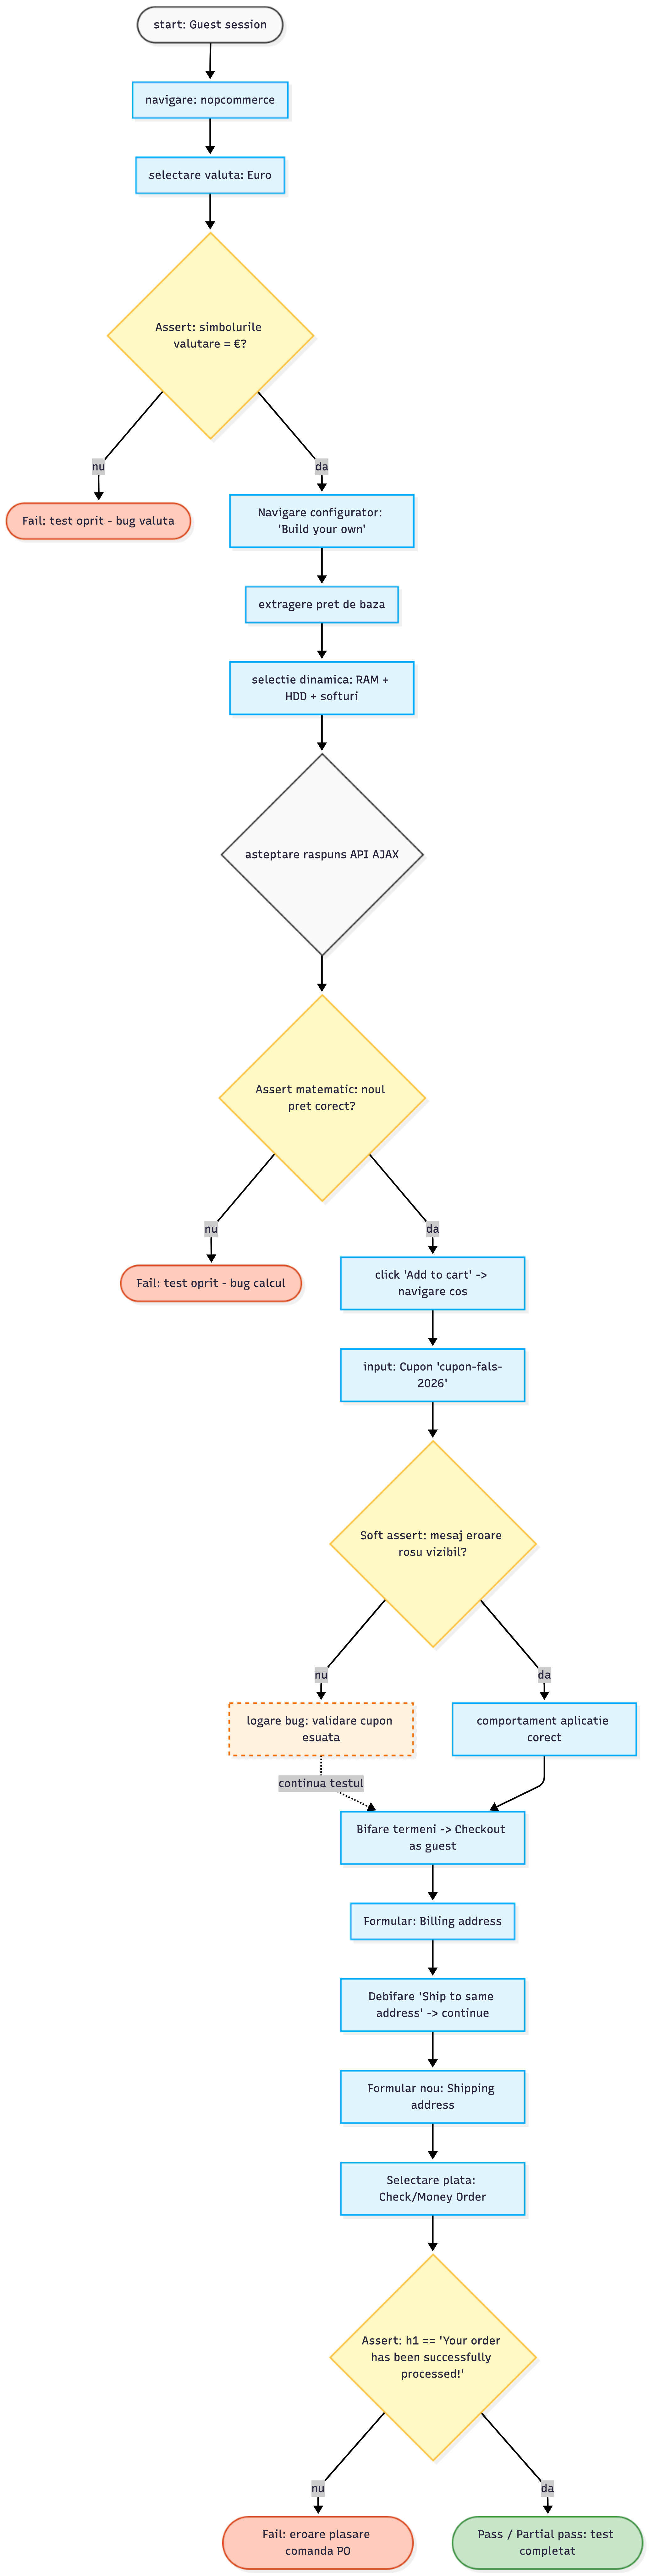
\includegraphics[width=0.3\textwidth]{diagrams/diagram2.png}
    \caption{Diagrama fluxului --- Workflow 2: Configurator PC}
    \label{fig:wf2}
\end{figure}

% -------------------------------------------------------
\section{Workflow 3 --- Tabelul de comparare produse}

\subsection*{Precondiții}
\begin{itemize}
    \item Sesiune fără autentificare.
    \item Lista de comparare este goală (fără rulări anterioare nesalvate).
\end{itemize}

\subsection*{Pași de testare}
\begin{enumerate}
    \item Căutare \textit{HTC} și adăugare la lista de comparare.
    \item Căutare \textit{Apple} și adăugare la lista de comparare.
    \item Navigare la pagina de comparare via banner-ul verde de notificare.
    \item \textbf{Assert}: tabelul HTML are exact 3 coloane.
    \item \textbf{Assert}: rândul de nume conține ambele produse.
    \item Click pe \textit{Clear list}.
    \item \textbf{Assert}: textul \textit{``You have no items to compare.''} este afișat.
\end{enumerate}

\begin{figure}[H]
    \centering
    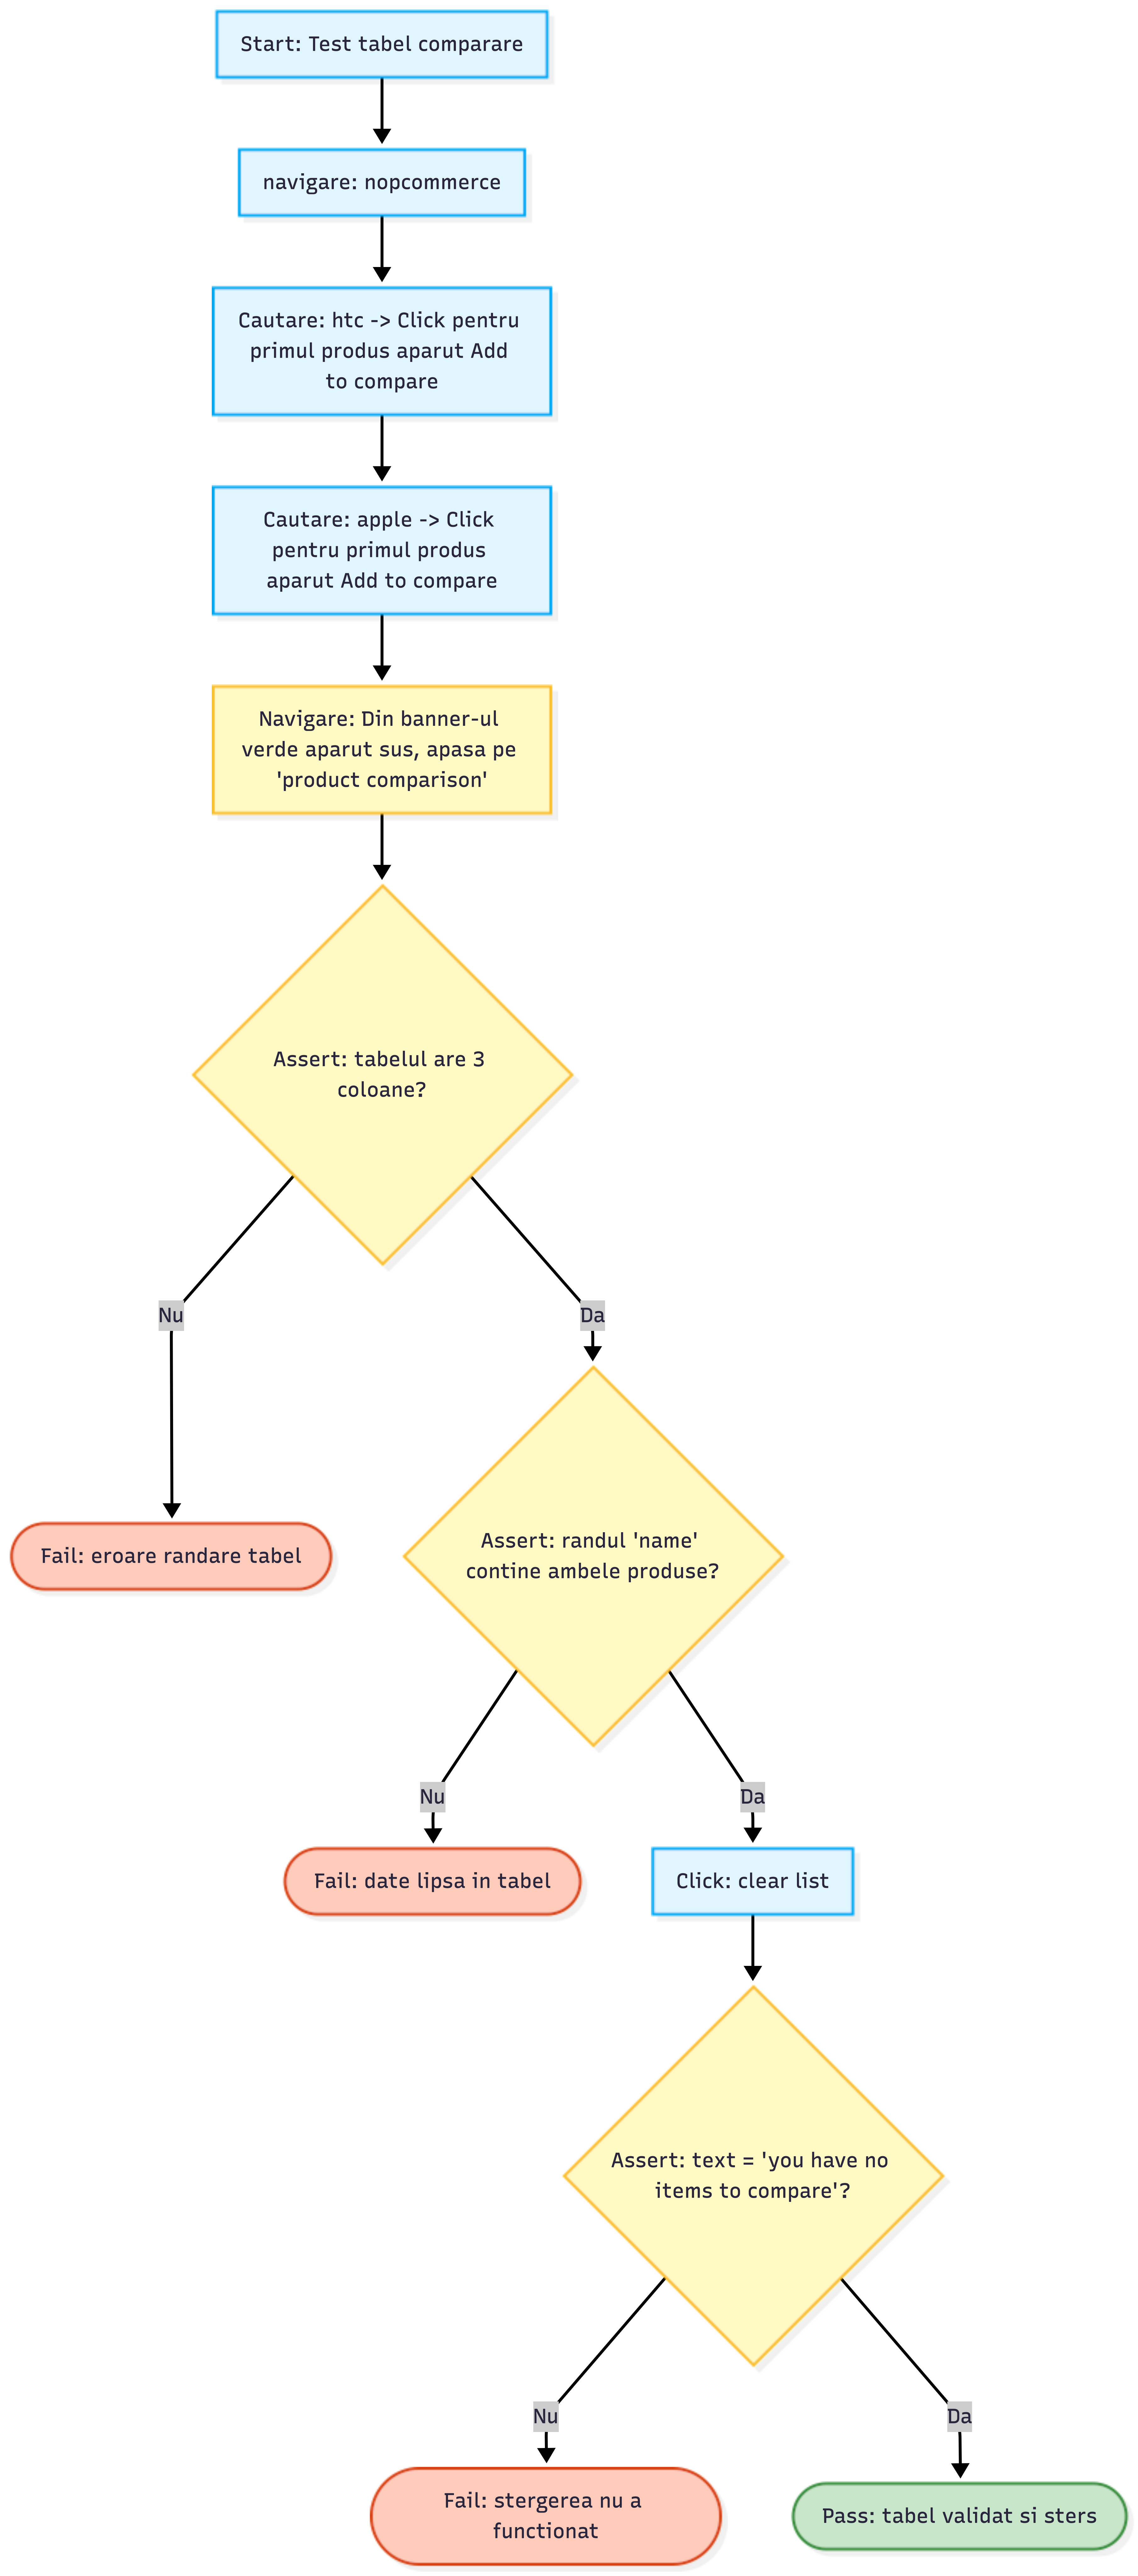
\includegraphics[width=0.3\textwidth]{diagrams/diagram3.png}
    \caption{Diagrama fluxului --- Workflow 3: Tabel comparare}
    \label{fig:wf3}
\end{figure}

% -------------------------------------------------------
\section{Workflow 4 --- Produs digital (livrare omisă)}

\subsection*{Precondiții}
\begin{itemize}
    \item Sesiune nouă de browser, coș gol, fără produse fizice în așteptare.
\end{itemize}

\subsection*{Pași de testare}
\begin{enumerate}
    \item Navigare la secțiunea \textit{Digital Downloads}.
    \item Adăugare album digital în coș.
    \item Checkout ca vizitator; completare adresă de facturare.
    \item \textbf{Soft assert}: pasul de livrare fizică este omis automat, iar tab-ul de plată devine activ direct.
    \item Selectare card ca metodă de plată; completare date fictive.
    \item \textbf{Assert}: mesaj de confirmare a comenzii virtuale.
\end{enumerate}

\begin{figure}[H]
    \centering
    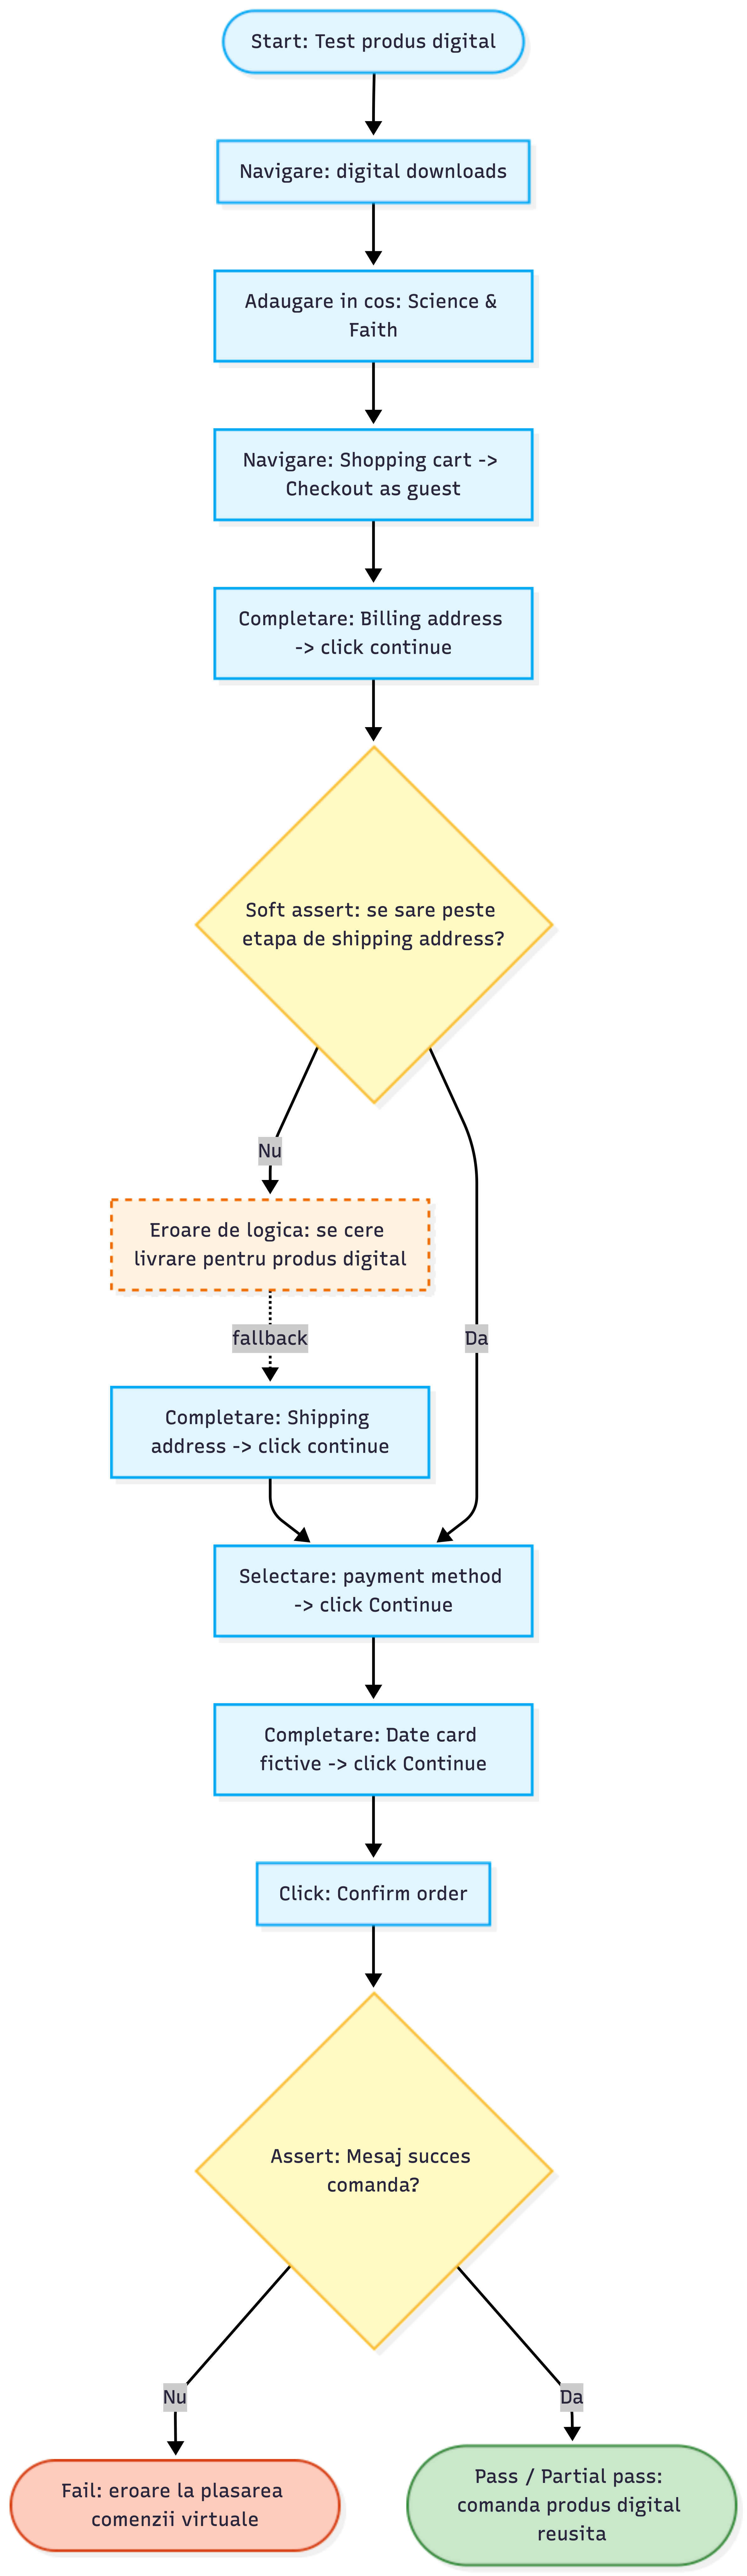
\includegraphics[width=0.3\textwidth]{diagrams/diagram4.png}
    \caption{Diagrama fluxului --- Workflow 4: Produs digital}
    \label{fig:wf4}
\end{figure}

% -------------------------------------------------------
\section{Workflow 5 --- Înregistrare cont și prima comandă}

\subsection*{Precondiții}
\begin{itemize}
    \item Scriptul generează un email unic la fiecare rulare prin concatenarea unui timestamp
          (\texttt{testuser\_\{timestamp\}@example.com}), evitând conflicte cu conturi existente.
\end{itemize}

\subsection*{Pași de testare}
\begin{enumerate}
    \item Navigare la formularul de înregistrare; completare date și email dinamic.
    \item \textbf{Assert}: mesajul \textit{``Your registration completed''} este afișat.
    \item Căutare produs \textit{Nokia Lumia} și adăugare în coș (utilizatorul este deja autentificat).
    \item Inițiere checkout.
    \item \textbf{Assert}: pasul de selecție \textit{login/guest} este omis --- contul tocmai creat este recunoscut automat.
    \item Completare adresă, metodă de livrare, plată cu card.
    \item \textbf{Assert}: URL conține \texttt{/checkout/completed} și mesajul de succes este afișat.
\end{enumerate}

\begin{figure}[H]
    \centering
    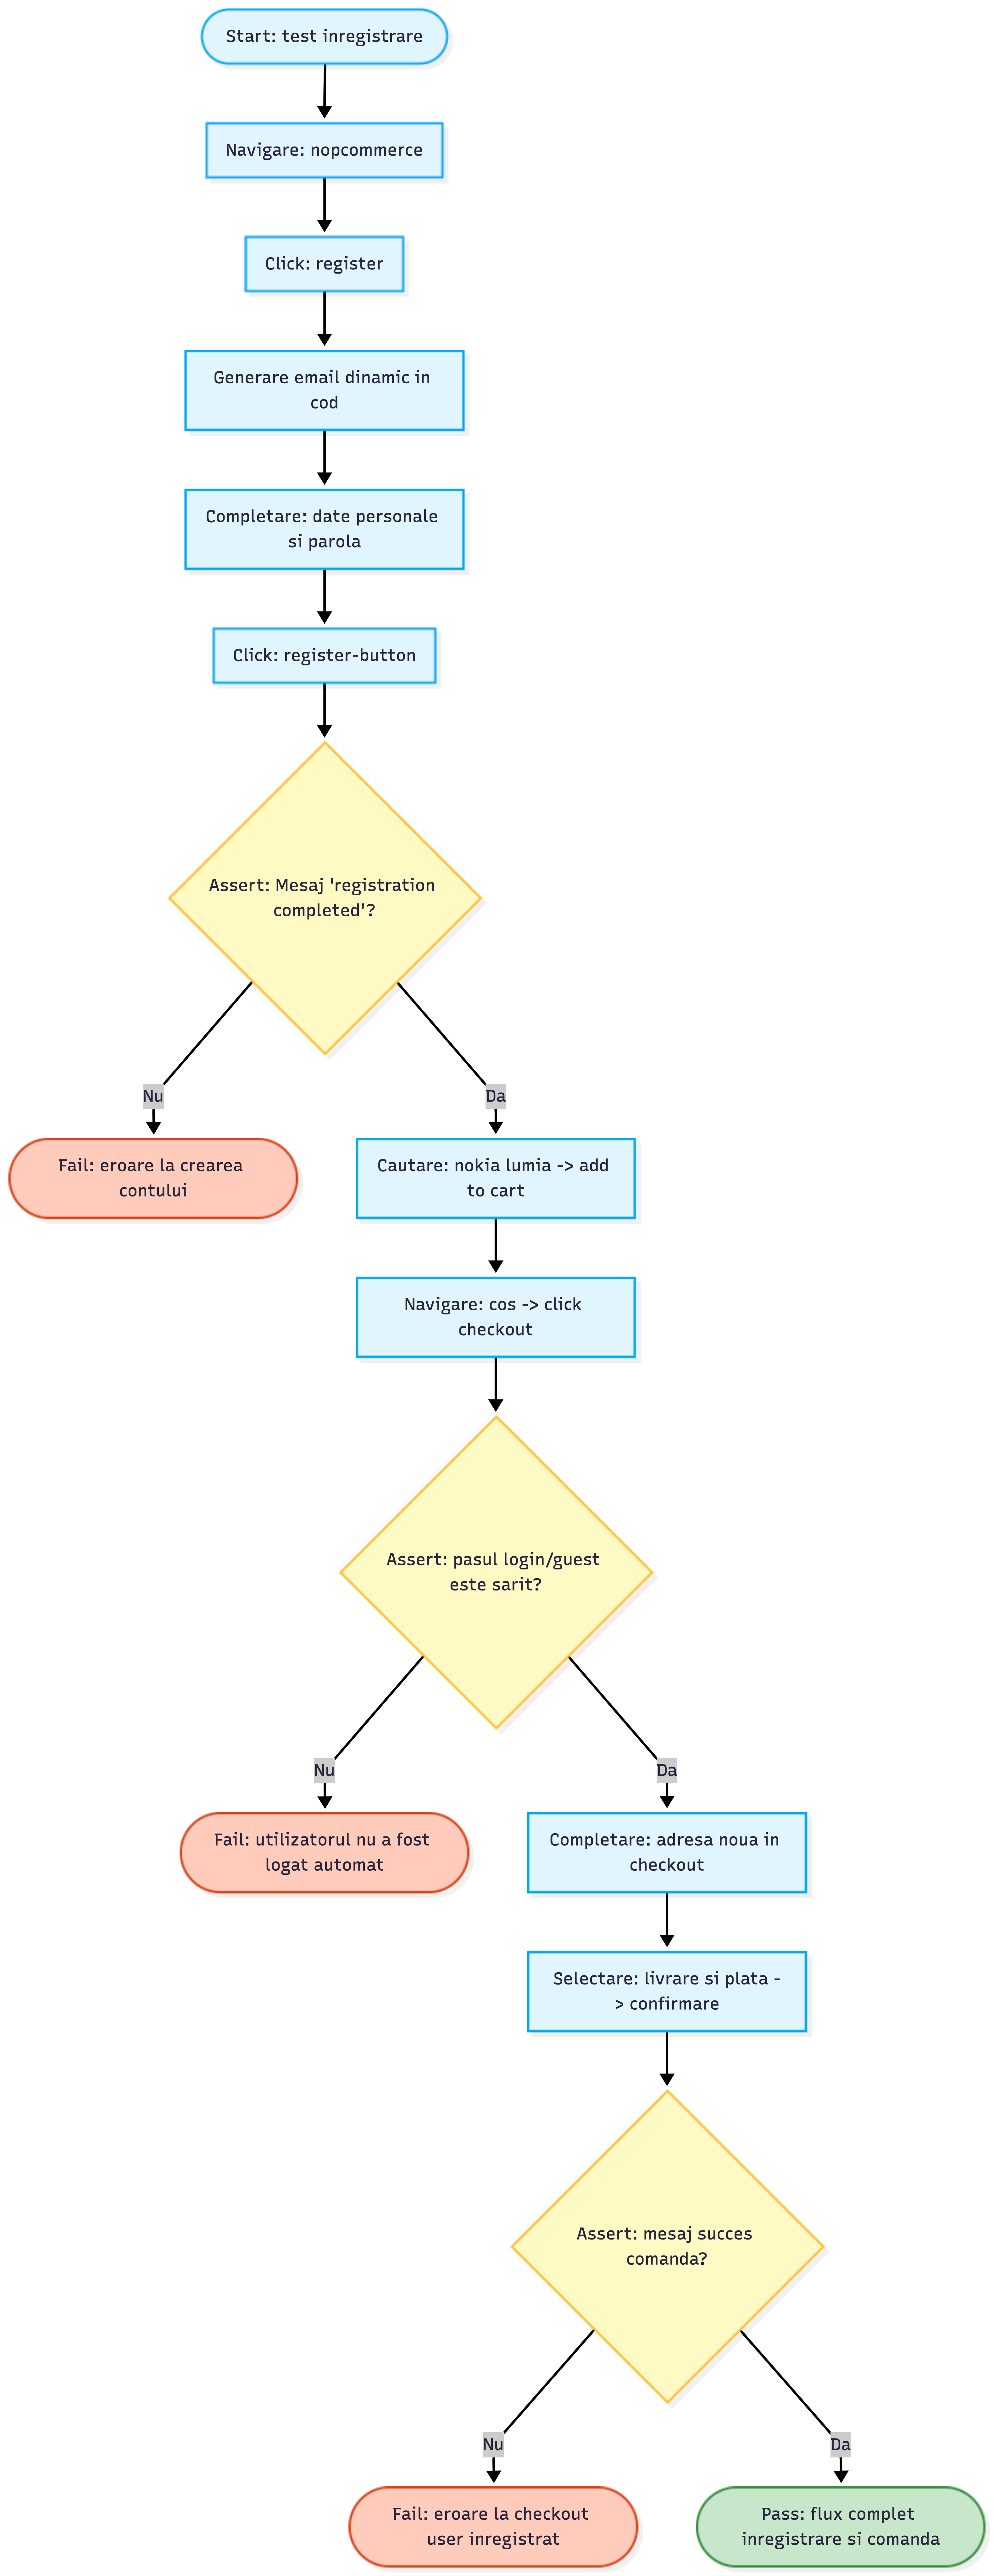
\includegraphics[width=0.3\textwidth]{diagrams/diagram5.png}
    \caption{Diagrama fluxului --- Workflow 5: Înregistrare și primă comandă}
    \label{fig:wf5}
\end{figure}

% -------------------------------------------------------
\section{Workflow 6 --- Persistența sesiunii (coș și adresă)}

\subsection*{Precondiții}
\begin{itemize}
    \item Există un cont persistent cu credențiale hardcodate în script
          (\texttt{persistent.tester2026@example.com}).
    \item Dacă nu există, scriptul îl creează automat înainte de test.
\end{itemize}

\subsection*{Pași de testare}
\begin{enumerate}
    \item Autentificare cu contul persistent.
    \item \textbf{Assert}: link-ul \textit{My account} este vizibil.
    \item Adăugare adresă nouă în agenda contului (cu un oraș generat dinamic).
    \item Adăugare produs \textit{Nokia Lumia} în coș.
    \item Deconectare (\textit{Log out}).
    \item \textbf{Assert}: link-ul de login a reapărut în header.
    \item Re-autentificare cu același cont.
    \item \textbf{Assert}: badge-ul coșului indică cel puțin un produs --- coșul a supraviețuit deconectării.
    \item Navigare la checkout.
    \item \textbf{Assert}: adresa salvată anterior apare în dropdown-ul de facturare.
\end{enumerate}

\begin{figure}[H]
    \centering
    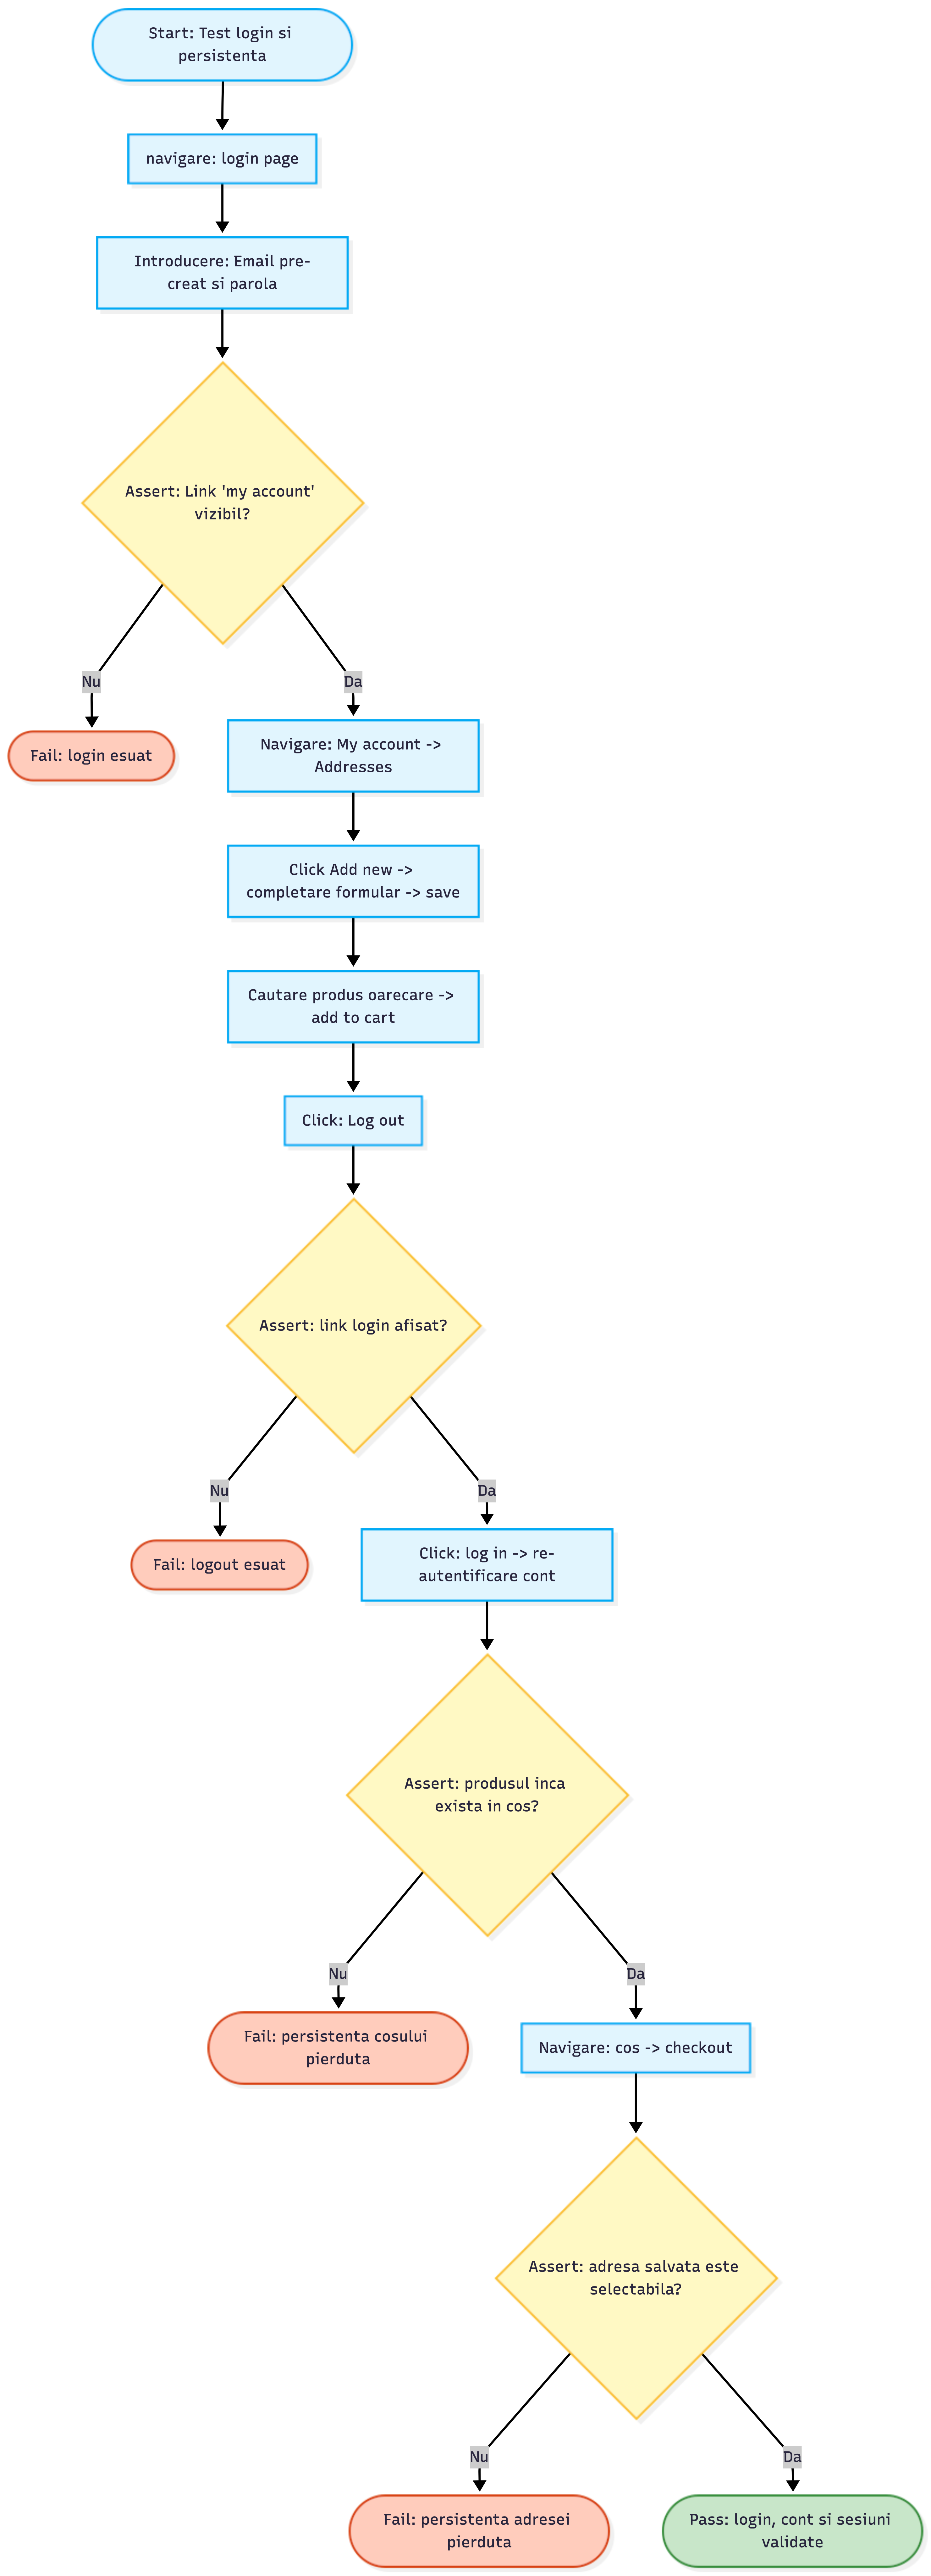
\includegraphics[width=0.3\textwidth]{diagrams/diagram6.png}
    \caption{Diagrama fluxului --- Workflow 6: Persistența sesiunii}
    \label{fig:wf6}
\end{figure}
